% Beamer talk — "Certifying Deep Learning Classifier Predictions with High Confidence"
% 6-8 minute MSc project video. Compile: cd paper && latexmk -pdf talk.tex
\documentclass[aspectratio=169]{beamer}
\usetheme{default}
\usecolortheme{seahorse}
\usepackage{graphicx}
\setbeamertemplate{navigation symbols}{}
\setbeamerfont{frametitle}{size=\large,series=\bfseries}
\title{Certifying Deep Learning Classifier Predictions\\with High Confidence}
\subtitle{A PAC-Bayes-with-Backprop study: MNIST \(\to\) Fashion-MNIST \(\to\) CIFAR-10}
\author{[Author]}
\institute{MSc Project, Department of Electrical \& Electronic Engineering}
\date{\today}
\begin{document}

\begin{frame}\titlepage\end{frame}

\begin{frame}{The problem}
\begin{itemize}
  \item Deep nets generalize well, but a test-set error gives \emph{no formal guarantee} about unseen data.
  \item We want a \alert{risk certificate}: a bound on the true error that holds with chosen confidence (e.g.\ 99\%).
  \item PAC-Bayes theory gives such certificates for \emph{probabilistic} nets (weights drawn from a learned distribution) --- but for decades they were \alert{vacuous} ($>1$) for deep nets.
\end{itemize}
\end{frame}

\begin{frame}{PAC-Bayes in one slide}
A stochastic predictor samples weights \(w\sim Q\). PAC-Bayes bounds the Gibbs risk \(R(Q)\) by the empirical risk plus a complexity term:
\[
R(Q)\;\lesssim\;\mathrm{kl}^{-1}\!\left(\hat R(Q)\;\Big\|\;\tfrac{\mathrm{KL}(Q\|P)+\log(2\sqrt n/\delta)}{n}\right)
\]
\begin{itemize}
  \item Tight when the posterior \(Q\) is \alert{close to the prior} \(P\) (small KL).
  \item \alert{Non-vacuous} requires (i) randomising the predictor (finite KL) and (ii) a prior near the posterior.
\end{itemize}
\end{frame}

\begin{frame}{PAC-Bayes-with-Backprop (P\'erez-Ortiz et al., 2021)}
Train \(Q\) by \emph{minimising a PAC-Bayes bound as the loss} (reparameterised, differentiable).
\begin{itemize}
  \item \textbf{Objectives:} \texttt{fquad}, \texttt{flambda} (tight relaxations) vs \texttt{fclassic} (looser) vs \texttt{bbb} (Bayes-by-Backprop, ELBO --- not a bound).
  \item \textbf{Priors:} data-free (\texttt{rand}) vs data-dependent (\texttt{learnt}, trained on a 50\% subset).
  \item \textbf{Predictors:} stochastic (what the cert bounds) / posterior-mean / ensemble (what you deploy).
\end{itemize}
\end{frame}

\begin{frame}{Setup: a difficulty ladder}
\begin{itemize}
  \item \textbf{MNIST} (reproduce P\'erez-Ortiz 2021, Table 1), \textbf{Fashion-MNIST} (new extension), \textbf{CIFAR-10} (analysis).
  \item FCN + CNN architectures; SGD, lr \(5\times10^{-3}\), \(\sigma_0=0.03\), 100 epochs; risk certificates by PAC-Bayes-\textit{kl} inversion.
  \item 26 runs total; every number traceable to a versioned run.
\end{itemize}
\end{frame}

\begin{frame}{MNIST reproduction: faithful}
Test errors reproduced within \(\le 0.4\)pp of the paper; the only gap is certificate looseness from a smaller MC budget. Key pattern:
\begin{itemize}
  \item \texttt{bbb}: best accuracy (2.0\% err) but loosest cert (0.61) --- it doesn't minimise a bound.
  \item \alert{Learnt prior tightens the \texttt{fquad} cert $\sim$8$\times$: 0.327 $\to$ 0.039}.
\end{itemize}
\end{frame}

\begin{frame}{Fashion-MNIST extension: the method transfers}
\begin{columns}[T]
\begin{column}{0.5\textwidth}
\begin{itemize}
  \item Same qualitative findings as MNIST.
  \item Learnt prior tightens the \texttt{fquad} cert $\sim$3$\times$: 0.429 $\to$ 0.145.
  \item Certificates stay non-vacuous on the harder task.
\end{itemize}
\end{column}
\begin{column}{0.5\textwidth}
\centering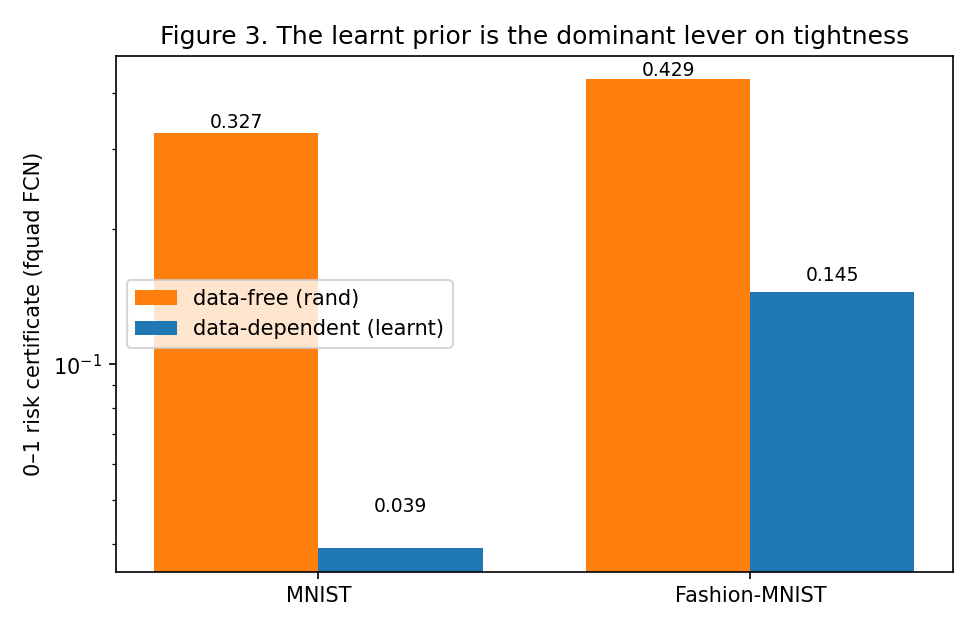
\includegraphics[width=\linewidth]{figures/prior.png}
\end{column}
\end{columns}
\end{frame}

\begin{frame}{Cross-dataset: certificate vs difficulty}
\begin{columns}[T]
\begin{column}{0.46\textwidth}
Learnt-prior \texttt{fquad} certificate rises \alert{monotonically} with task difficulty:
\[0.039 \to 0.145 \to 0.410\]
Informative on MNIST/Fashion-MNIST; approaching vacuity on CIFAR-10 --- driven by irreducible error.
\end{column}
\begin{column}{0.52\textwidth}
\centering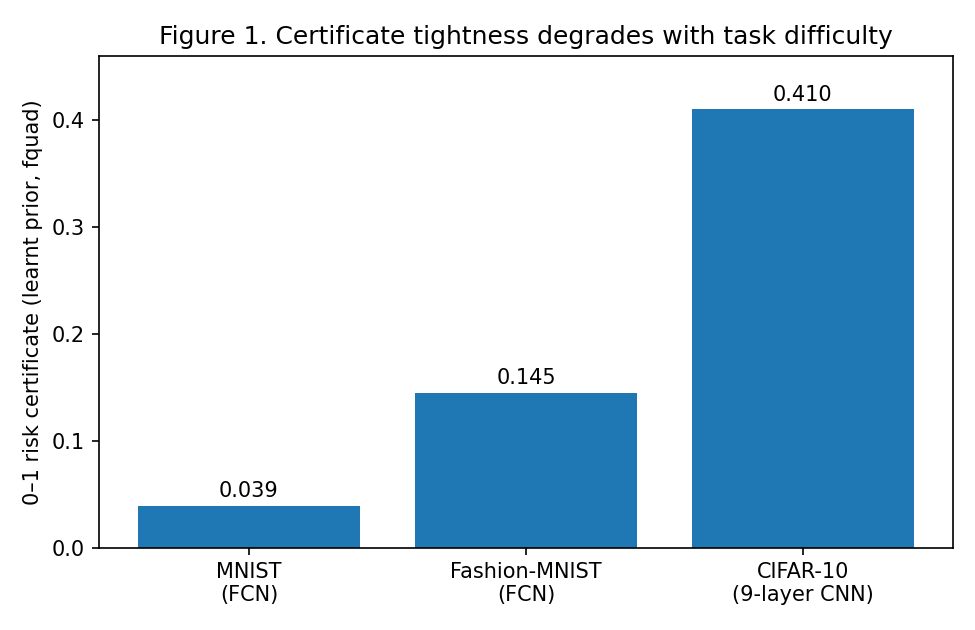
\includegraphics[width=\linewidth]{figures/ladder.png}
\end{column}
\end{columns}
\end{frame}

\begin{frame}{Small-data: bound stays non-vacuous at 10\% data}
\begin{columns}[T]
\begin{column}{0.46\textwidth}
Self-certified bound degrades \alert{gracefully}: data $\times\frac{1}{10}$, cert only $\sim\times2$ (0.039 $\to$ 0.072, still $\ll 1$).
\end{column}
\begin{column}{0.52\textwidth}
\centering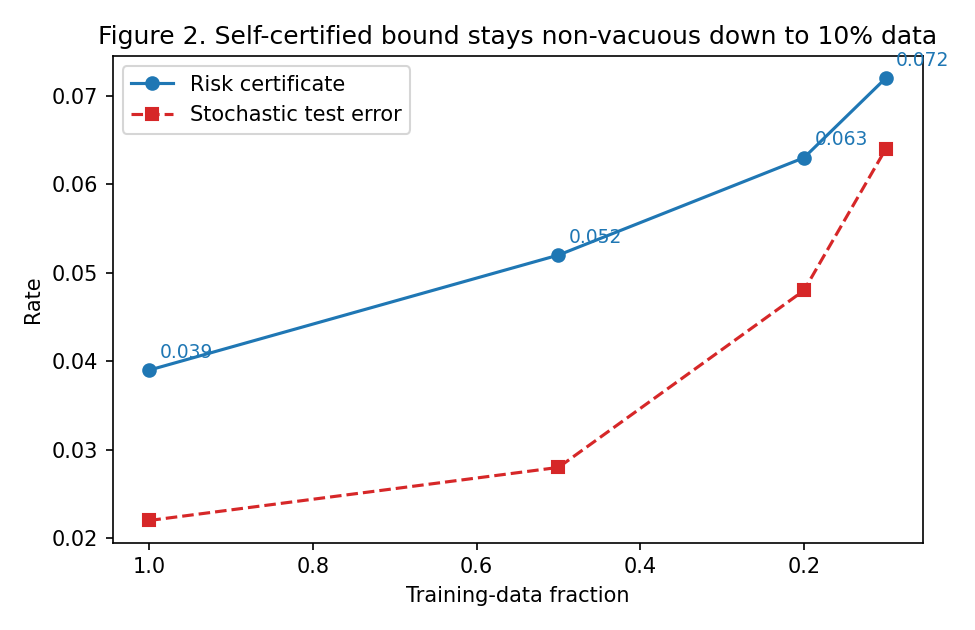
\includegraphics[width=\linewidth]{figures/smalldata.png}
\end{column}
\end{columns}
\end{frame}

\begin{frame}{Takeaways}
\begin{itemize}
  \item \alert{Bound-minimising training works}: competitive accuracy \emph{and} non-vacuous certificates.
  \item \alert{The prior is everything}: data-dependent priors are the largest lever on tightness.
  \item Certificates track difficulty (informative $\to$ vacuous across the ladder); the self-certified bound is data-efficient.
  \item Open question: a certificate \emph{valid for the deployed (mean) predictor}, not just the stochastic one.
\end{itemize}
\end{frame}

\begin{frame}{Thank you / Questions}
\centering Report + code + 26 runs: \texttt{pacbayes-cert}\\[1em]
Reference reproduced: P\'erez-Ortiz et al., \emph{JMLR} 2021 (arXiv:2007.12911).
\end{frame}

\end{document}
